\chapter{Implementering}

\subsection{Brugergrænseflade}
Ved programmets opstart vises det statiske kort som gruppen har valgt at benytte under udviklingen af dette program, samt en load knap. Dette er at finde i tabben “Map View”. Tabben “Data View” vil ikke indeholde noget information ved opstart af programmet. Efter tryk på load knappen, popper en dialogbox op, hvorefter brugeren skal vælge den mappe som indeholder løbernes GPX-filer, samt koordinater for posterne til den bane løberne skal løbe. Dette kan ses på figur 7.1.

\begin{figure} [h]
	\centering
	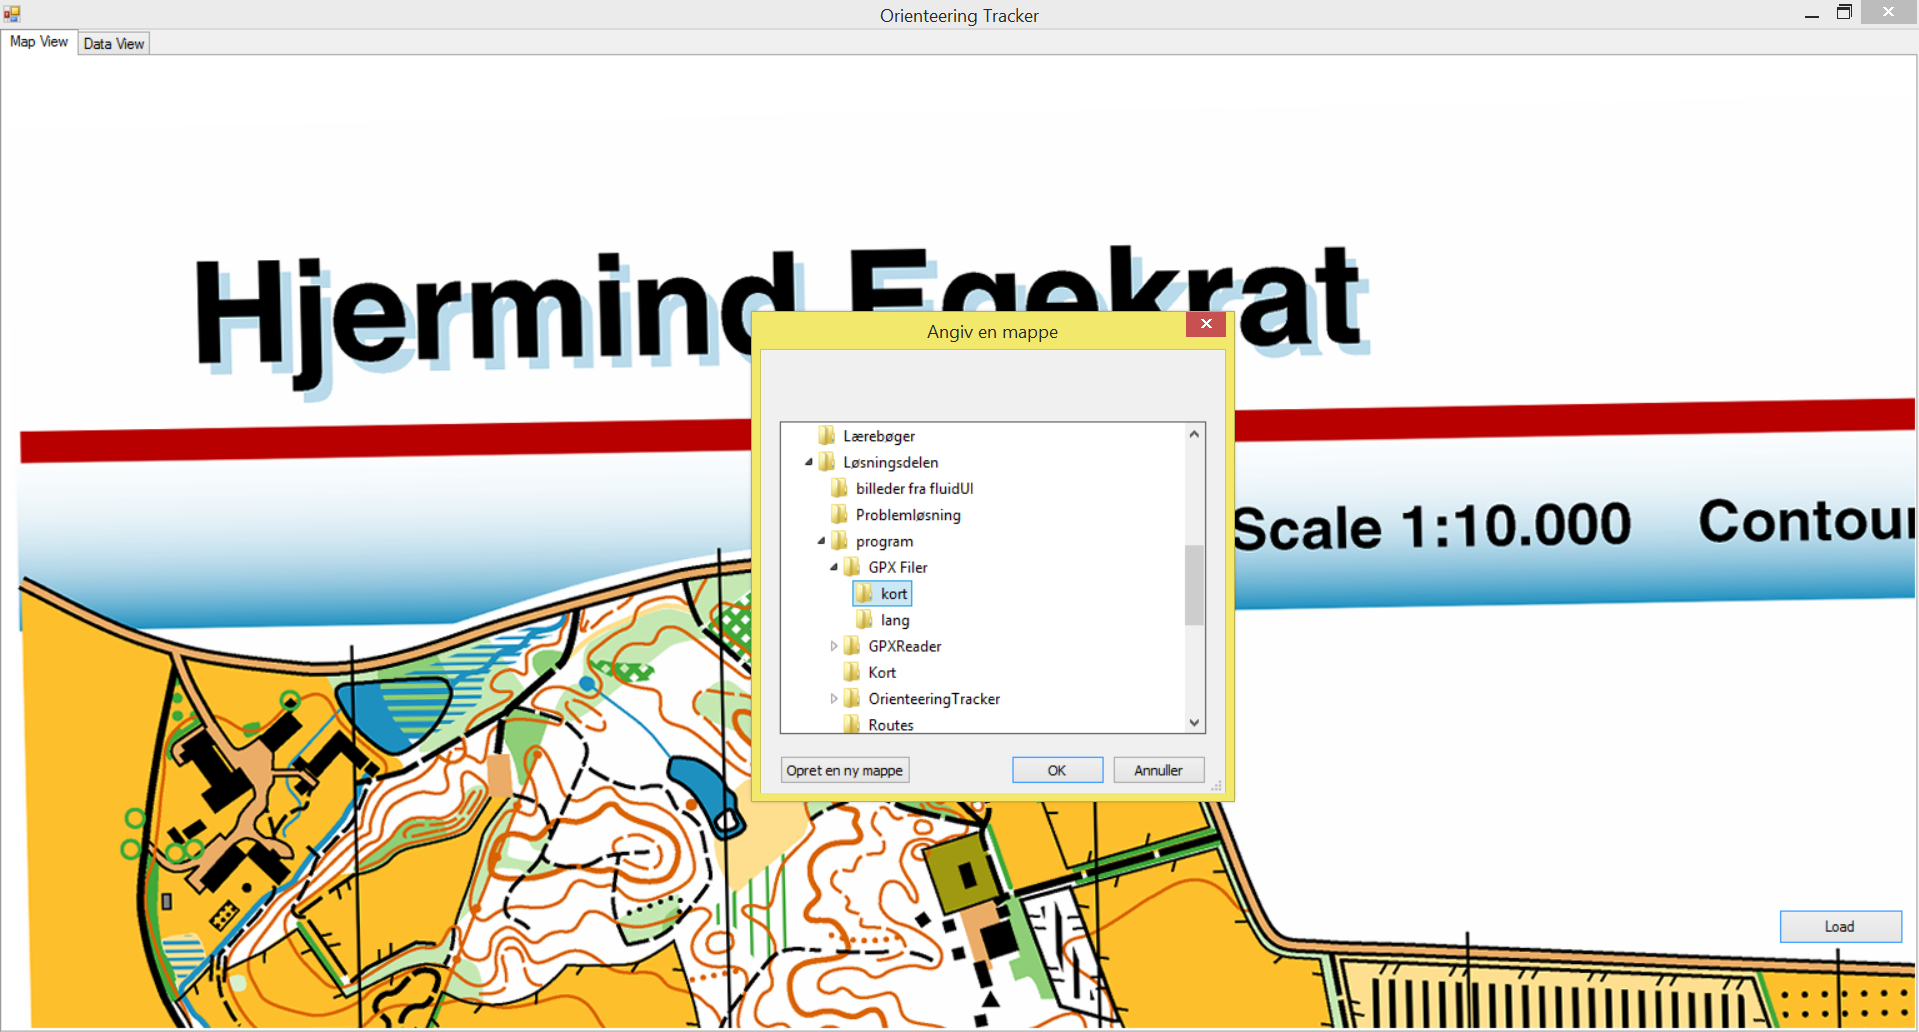
\includegraphics[width=1\textwidth]{billeder/MapView1}
	\caption{Klassediagram over projektets program}
\end{figure}

Når GPX-filer og koordinaterne for posterne er loadet ind i programmet, vil de forskellige mediaplayer funktioner komme frem, som ses på figur 7.2.

\begin{figure} [h]
	\centering
	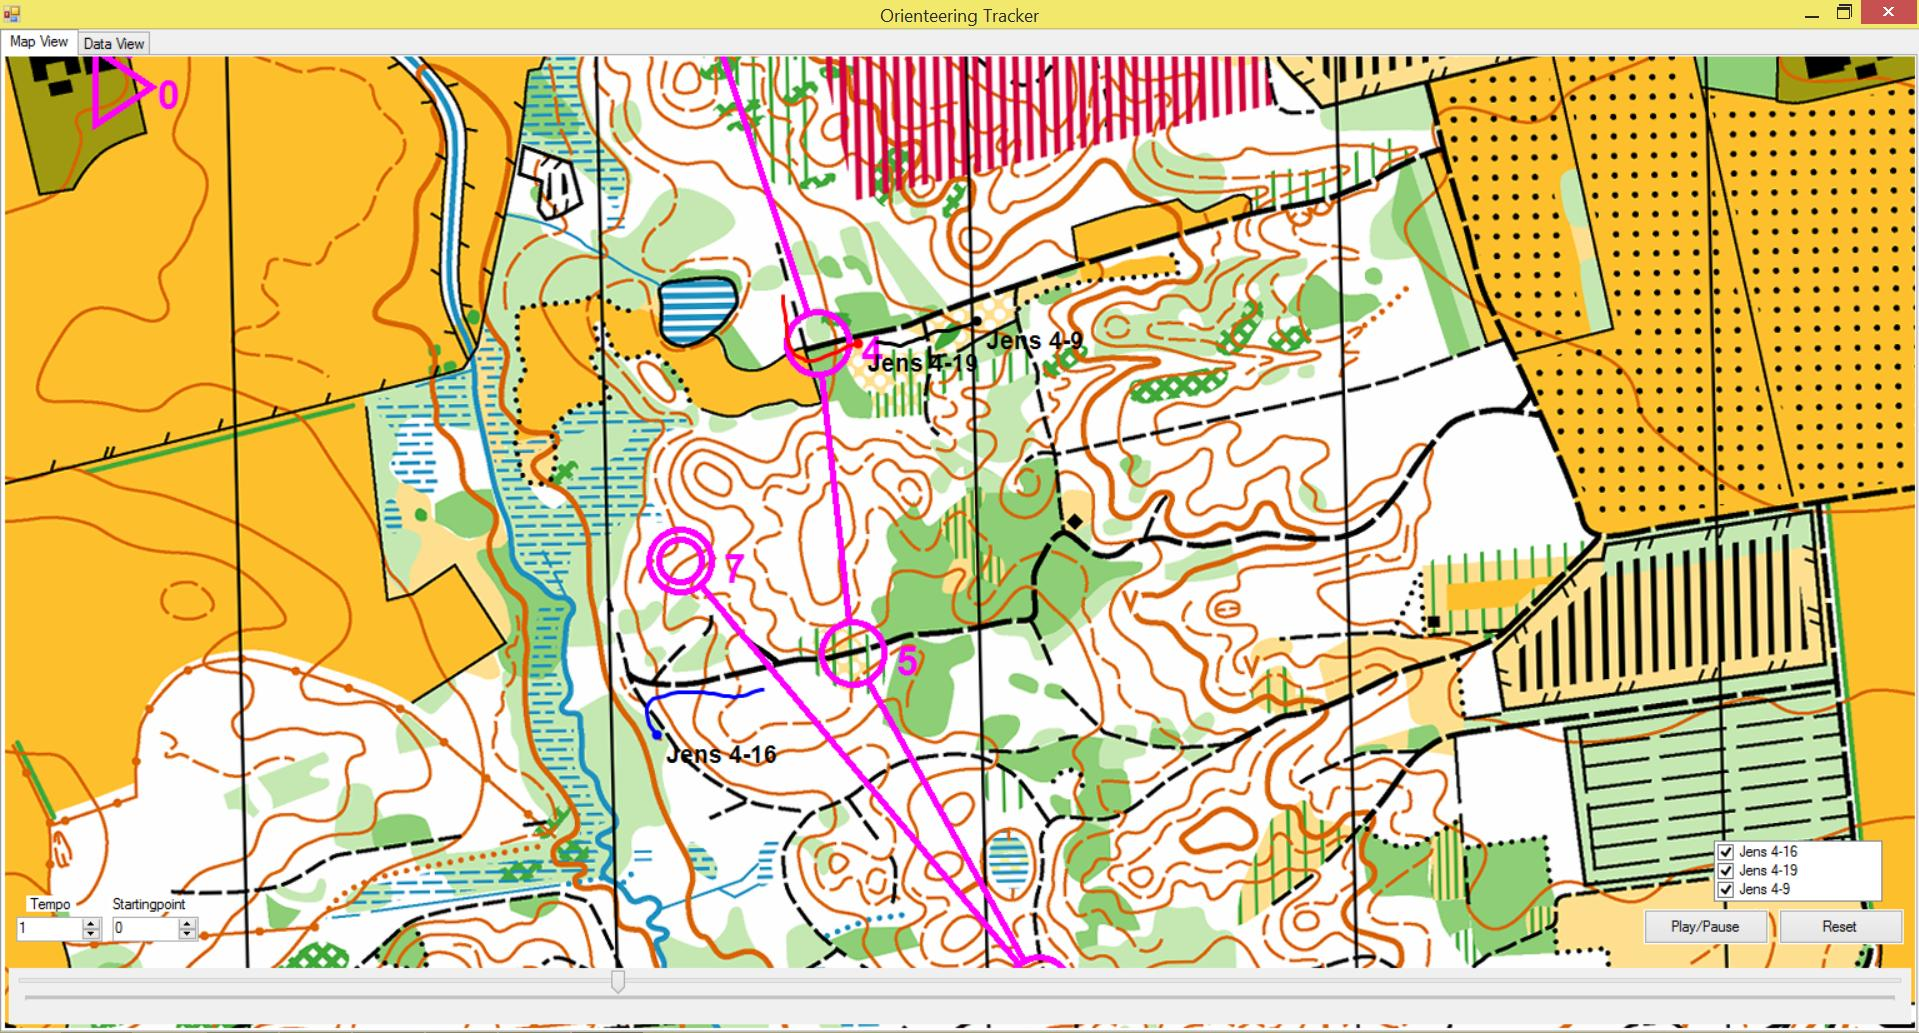
\includegraphics[width=1\textwidth]{billeder/MapView2}
	\caption{Klassediagram over projektets program}
\end{figure}

I bunden af programmet ses programmets trackbar, der gør det muligt at spole frem og tilbage under afspilningen. Nede i venstre hjørne findes to forskellige mediaplayer funktioner. Den yderste til venstre bruges til at vælge tempoet for afspilningen. Den anden bruges til at vælge startpost for løberne, hvilket gør det muligt at samle løberne, for lettere at kunne sammenligne dem med hinanden. På højre side ses en play/pause og  reset knap. Play/pause bruges til at starte/pause afspilningen. Reset knappen bringer programmet tilbage til dets opstarts stadie. Lige over disse to knapper findes en check box. I denne checkbox kan alle løberne ses. Checkboxen afgør hvilke løbere der vises på kortet, hvilket gør det muligt at skjule løbere, hvis der vil fokuseres på nogle bestemte løbere. Løberne vises ude på kortet med en prik i hver deres farve, samt en hale efter denne, som viser hvordan de har løbet de sidste 30 sekunder. 

Når der trykkes på tabben “Data View” vil alle løbernes data for løbet vises. I “Data View” kan der ses løbernes slut position, navn, tid, tidsdifference til førstepladsen, tilbagelagt distance, hastighed i minut pr. kilometer og tiden for hvert stræk. Der kan ses et eksempel på dette på figur 7.3 herunder. 
\begin{figure} [h]
	\centering
	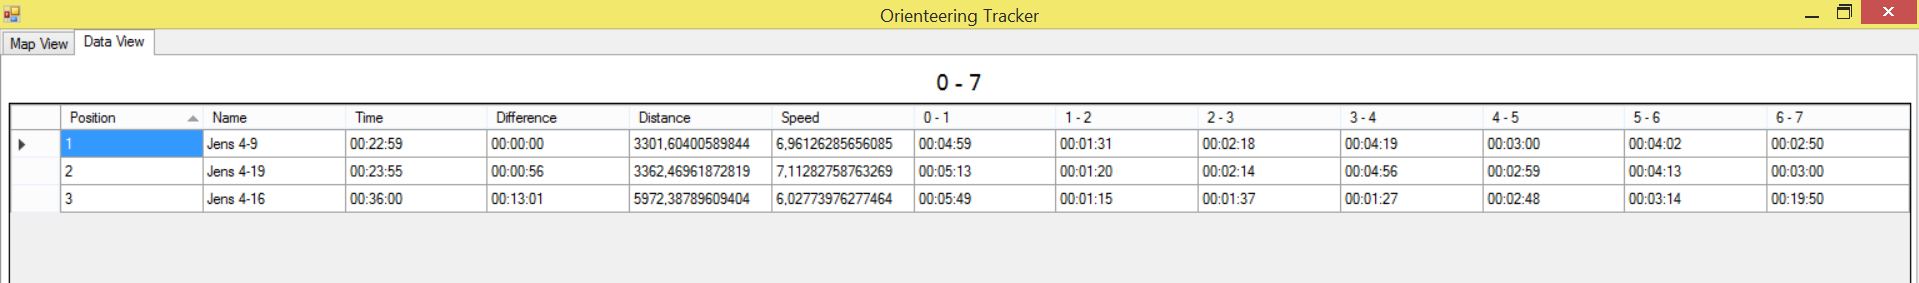
\includegraphics[width=1\textwidth]{billeder/DataView1}
	\caption{Klassediagram over projektets program}
\end{figure}

Klikkes der på et felt for et stræk, kan der ses mere detaljerede informationer om det specifikke stræk. Som det kan ses på figur 7.4, indeholder dette de samme informationer som når der ses på hele løbet, med en enkelt undtagelse, her kan løberne se hvilken position de fik på det specifikke stræk. 
\begin{figure} [h]
	\centering
	\includegraphics[width=1\textwidth]{billeder/DataView2}
	\caption{Klassediagram over projektets program}
\end{figure}

\section{Programstruktur}
Da ingen af medlemmerne i gruppen har tidligere erfaring med udvikling af store applikationer i C\# og Windows Forms, blev meget af udviklingen lavet ud fra “trial and error” princippet. Med det menes at gruppen forsøgte sig meget frem, for at lære at bruge Windows Forms, og der ikke blev lavet en decideret plan eller design for programmet, før udviklingen blev påbegyndt. Dette medførte at store dele af programmet blev lavet i samme klasse, hvilket forårsagede et forholdsvist lavt abstraktionsniveau. 

\subsection{Klassebeskrivelse}
Gruppen har vha. Visual Studio udarbejdet et klasse diagram, for at give et bedre overblik over programmets klasser. I firkanterne i klassediagrammet ses klassens navn, dens fields, properties og metoder.

\begin{figure} [h]
	\centering
	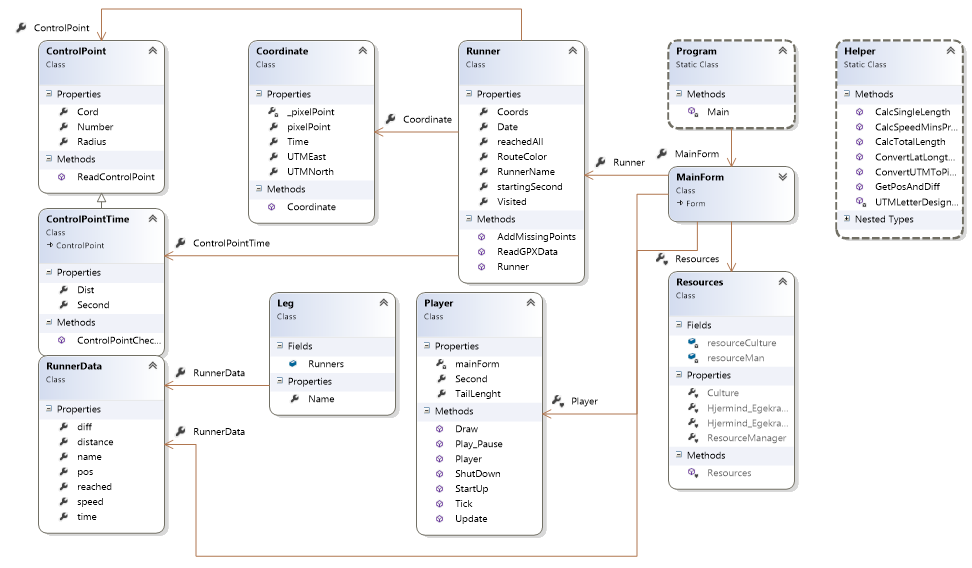
\includegraphics[width=1\textwidth]{billeder/KlasseDiagram}
	\caption{Klassediagram over projektets program}
\end{figure}

\begin {itemize}
\item \textbf{Helper} klassen indeholder de metoder der bruges til at lave udregninger i programmet, eksempelvis konverteringen fra længde- breddegrade koordinater til UTM koordinater. 
\item \textbf{Coordinate} indeholder koordinater for at kunne se hvor løberen er og hvor posterne er placeret, som både pixel- og UTM koordinater. 
\item \textbf{ControlPoint} repræsentere posterne i løbet. Hvor den indeholder en posts radius, dens nummer og henter dens koordinater fra Coordinates.
\item \textbf{ControlPointTime} har nedarvet fra ControlPoint, hvor den så implementere Second og Dist som vil være tid i sekunder og distancen fra løberen til posten. 
\item \textbf{Runner} indeholder informationer om en løber, dette er bl.a. løberens koordinater på ruten, om løberen har besøgt alle poster og løberens navn.
\item \textbf{RunnerData} gemmer på en mængde data om hver enkelt løber, som hastighed, distance løbet og position i løbet, hvor dette vil være de informationer som kan findes under tabben som gruppen har kaldt ”Data view”. 
\item \textbf{Leg} er det som førnævnt kaldet et ”stræk”, dog nu oversat til engelsk. Leg indeholder en list af RunnerData samt et navn på strækket.
\item \textbf{Player} sørger for at tegne løberen på kortet, samt den hale som skal være efter løberen. Derudover viser, skjuler og opdatere den forskellige funktioner i programmet når det køres, dette bruges i den tab som gruppen har kaldt ”Map view”.
\item \textbf{MainForm} holder sammen på programmet. Det er er GUI’en bliver lavet, samt events til programmet. 
\item \textbf{Resources} indeholder kortet som bruges I programmet, samt worldfilen.
\end {itemize}


